%%%%%%%%%%%%%%%%%%%%%%%%%%%%%%%%%%%%%%%%%%%%%%%%%%%%%%%%%%%%%%%%%%%%
%% MMRFIC Document template header v0.1
%%
%% (C) MMRFIC Technology Pvt. L:td., Bangalore.
%%
%%  NOTE:
%%  This header needs to be kep as it is for all LaTeX documents.
%%  If you have any comments, please send them to gana@mmrfic.com 
%%%%%%%%%%%%%%%%%%%%%%%%%%%%%%%%%%%%%%%%%%%%%%%%%%%%%%%%%%%%%%%%%%%%
%% Header starts from here  <<<<<<<<<<<<<<<<<<<<<<<<<<<<<<<<<<<<<<<<

\documentclass[12pt,a4paper,onecolumn]{article}
\usepackage[utf8]{inputenc}
\usepackage[english]{babel}
\usepackage{amsmath}
\usepackage{amsfonts}
\usepackage{amssymb}
\usepackage{graphicx}
\usepackage[left=2.5cm,right=2.5cm,top=3cm,bottom=3cm]{geometry}
\author{MMRFIC Technology Pvt. Ltd., Bangalore}
\title{Fountain Code}

\usepackage{fancyhdr}
\pagestyle{fancy}
\usepackage{lastpage}

%% Header and footer style
\lhead{}
%\chead{}
%\rhead{}
%\lfoot{}
%\cfoot{}
%\rfoot{}

\fancyhead{}  % Cleal default format
\rhead{MMRFIC Confidential: NDA Required}
\fancyfoot{}  % Cleal default format
%\fancyfoot[LE,RO]{\thepage}           
%\fancyfoot[RO]{Page \thepage\ of\  \pageref{\LastPage}}           % page number
\fancyfoot[RO]{Page \thepage}           
% page number in "outer"positionfooterline
\renewcommand{\headrulewidth}{0.4pt}
\renewcommand{\footrulewidth}{0.6pt}
\setcounter{figure}{0}
\makeatletter
\renewcommand{\thefigure}{\@arabic\c@figure}
\makeatother 

%% Watermark
%\usepackage[firstpage]{draftwatermark}
\usepackage{draftwatermark}
\SetWatermarkFontSize{10cm}
\SetWatermarkColor[rgb]{100}
%\SetWatermarkText{VER 0.1}
\SetWatermarkText{VER 0.1}
\SetWatermarkLightness{0.5}

%% Other misc used in the project
\usepackage{longtable}
%% Header ends from here  >>>>>>>>>>>>>>>>>>>>>>>>>>>>>>>>>>>>>
%% 
%% NOTE2:
%% After copying the header lines, do not change the order of the lines.
%% Make changes only to title of the document, Watermark text (including the 
%% version number of the document, and rhead{} content. Allowed rhead{} lines 
%% are  (i) \rhead{MMRFIC Confidential: NDA Required}, (ii) \rhead{MMRFIC 
%% Tutorial}, (iii) \rheaf{}


\begin{document}
%\title{User Guide for RF Driver Board V0.2}
\maketitle
\vfill

\begin{table}[h]
\begin{center}
\begin{tabular}{llll}
\hline
Ver. & Author(s) & Date & Comments \\
\hline \hline
1.0 & Sudhanshu Sharma & 19/11/2019 & created \\%%% Enter version history here
\hline
\end{tabular}
\caption{Version History}
\end{center}
\end{table}
\newpage
\tableofcontents
\newpage
\section{Introduction}
This document contains the implementation of fountain codes. It explains encoding, decoding, channel information, modulation and demodulation for a given set of information.
\section{Input Data}
Input is 63 x 1 matrix which is in binary format (1's, 0's). It is 63 because of the columns in code matrix. 
\section{Encoder}
Here we are using CodeMatrix for encoding and decoding, information about code matrix is presented at both the transmitter and receiver end. Size of Code matrix for this particular experiment was given as  441 x 21 (In octal format) which was then converted into 441 x 63 (Binary Format) as we are using Galois Field 2 which has only 0 and 1.Each row of code matrix will have only 3 non- zero elements.\\
Encoding is done by multiplying the input with the code matrix. Hence the size of code matrix is 441 x 63 so we have chosen input size as 63 x 1 which yield the Encoded output Bits as 441 x 1.
\begin{center}
\begin{equation}
\begin{bmatrix}
p_{1,1} & p_{1,2} & \ldots
& p_{1,63} \\
p_{2,1} & p_{2,2} & \ldots
& p_{2,63} \\
\vdots & \vdots & \ddots
& \vdots \\
p_{441,1} & p_{441,2} & \ldots
& p_{441,63}
\end{bmatrix}
\end{equation}

\end{center} 
\section{Modulation}
Here we are doing BPSK in which the bit 0 is mapped to bit -1 and bit 1 is mapped to 1. 
After the modulation we have to pass the symbols to the channel 
\section{Channel Error}
We are using two different channels - %
\begin{enumerate}
\item BSC (Binary Symmetric Channel) : In this model, a transmitter wishes to send a bit (a zero or a one), and the receiver receives a bit. It is assumed that the bit is usually transmitted correctly, but that it will be "flipped" with a small probability (the "crossover probability"). \\
So here it’s like - for block size 180 we had Error Probability of 1e-6, 1e-5, 1e-4, 1e-3, 1e-2. And then for block size 220, again Error Probability of 1e-6, 1e-5, 1e-4, 1e-3, 1e-2 and so on. 
\item
Additive White Gaussian Noise : Additive white Gaussian noise (AWGN) is a basic noise model used in Information theory to mimic the effect of many random processes that occur in nature. 
\\
\end{enumerate}
Calculation of Sigma was done for all the SNR values from 1 to 10. Then added to the modulated signal.\\
\begin{equation*}
\sigma = \sqrt{\frac{1}{10^\frac{SNR(ErrorPro)}{10}}}x
\end{equation*}
\\
It was similar to BSC in the ways of implementation like - \\
We did AWGN channel Model  with SNR of 1 to 10 .And with the block size of 180 to 300 in- steps of 40.
\section{Demodulation}
Demodulation is done using LLR (Log -Likelihood Ratio)
\begin{equation*}
\rho = \log(\frac{P(y|b(w)=0,r)}{P(y|b(w)=1,r)})
\\
\end{equation*}
\begin{equation*}
= \log(\frac{\sum_{x0} P(y|w,r)}{\sum_{x1} P(y|w,r)} )
\end{equation*}
\begin{equation*}
P(y|w,r) = \frac{1}{\sqrt{2\pi\sigma^2}}.\exp(\frac{-(y-rw^2)}{2\sigma^2})
\end{equation*}
\begin{equation*}
\rho = \frac{2ry}{\sigma^2}
\end{equation*}
\\
Hence we can clearly see that it depends on the “ry” value if ry is positive the demodulated output is going to be positive and if its negative that the result is negative.
Which is done using \\
\begin{center}
$Demoded = (1*(ChannelOutput > 0));$
\end{center}

\section{Decoder }
Decoding is done using Gaussian Elimination in which Demodulated bits are augmented with Code Matrix 

\begin{equation*}
\begin{bmatrix}
CodeMatrix_{1,1} & CodeMatrix_{1,2} & \ldots
& CodeMatrix_{1,63} \vert & DemodulatedBits_{1,64} \\
CodeMatrix_{2,1} & CodeMatrix_{2,2} & \ldots
& CodeMatrix_{2,63} \vert & DemodulatedBits_{1,64} \\
\vdots & \vdots & \ddots
& \vdots  & \vdots \\
CodeMatrix_{441,1} & CodeMatrix_{441,2} & \ldots & CodeMatrix_{441,63} \vert & DemodulatedBits_{441,64}
\end{bmatrix}
\end{equation*}

Out of available 441 x 64 random rows are selected for different block size. As we only need K+E bits to do Gaussian Elimination where K - size of input and E - Extra bits to perform Gaussian Elimination
\\
\\
Gaussian Elimination Algorithm 
\\M - Rows , N - Columns
\begin{enumerate}
\item Search for 1’s column wise.
\begin{itemize}
\item IF no 1s’ are found, report - “lack of 1’s to perform Gaussian Elimination”. And give output as all zeros.
\item ELSE make the First encountered 1 as First row of the matrix
\end{itemize}
\item Then XOR with next 1’s found on that same column to make it zero.
\item Performing this for all N will yield square matrix with all diagonal as 1’s and all the element below diagonal as zeros.And are the non redundant element below the square (Upper triangular matrix)
\item By back substituting from nth row and  keep solving the equation by equating it to the nth element.
\end{enumerate}
\section{Modification/cases}
Initially, We were using all 441 rows to solve for Gaussian Elimination and then we start using random rows of particular block size to solve for Decoded output bits.
\\
Then later we sorted the received symbols (after AWGN channel) in increasing order of the signal amplitude and picked the top “BlockSize” rows from there. Then used the BlockSize to decode the payload. And which result in better BER vs SNR curve. 
\newpage
\section{Results}
Figure \ref{BSC_Channel} Result of BSC Channel (Error Probability vs BER)
Figure \ref{AWGN_Channel} Result of BSC Channel (Error Probability vs BER)

\begin{figure}[htb]  
\vspace{-0.1in}
  \begin{center}
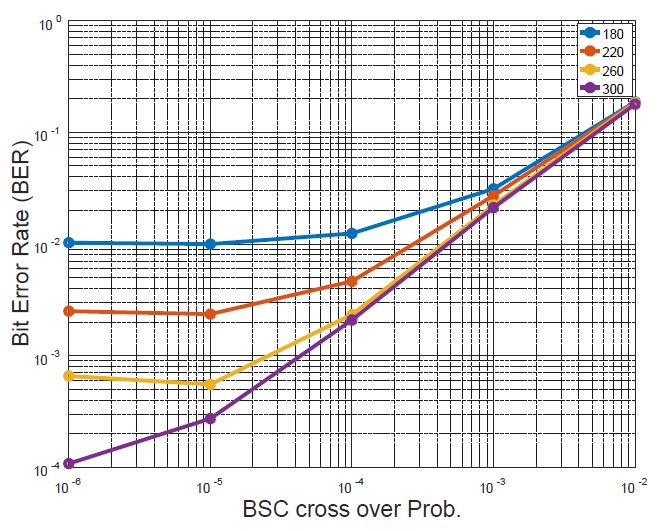
\includegraphics[scale=0.4]{BSC.JPG} 
\caption{Result of BSC Channel (Error Probability vs BER)}
\label{BSC_Channel}
 \end{center}
\vspace{-0.1in}
%\caption{DSP Firmware State machine.}
%\label{fig:statemc}
\end{figure}

\begin{figure}[htb]  
\vspace{-0.1in}
  \begin{center}
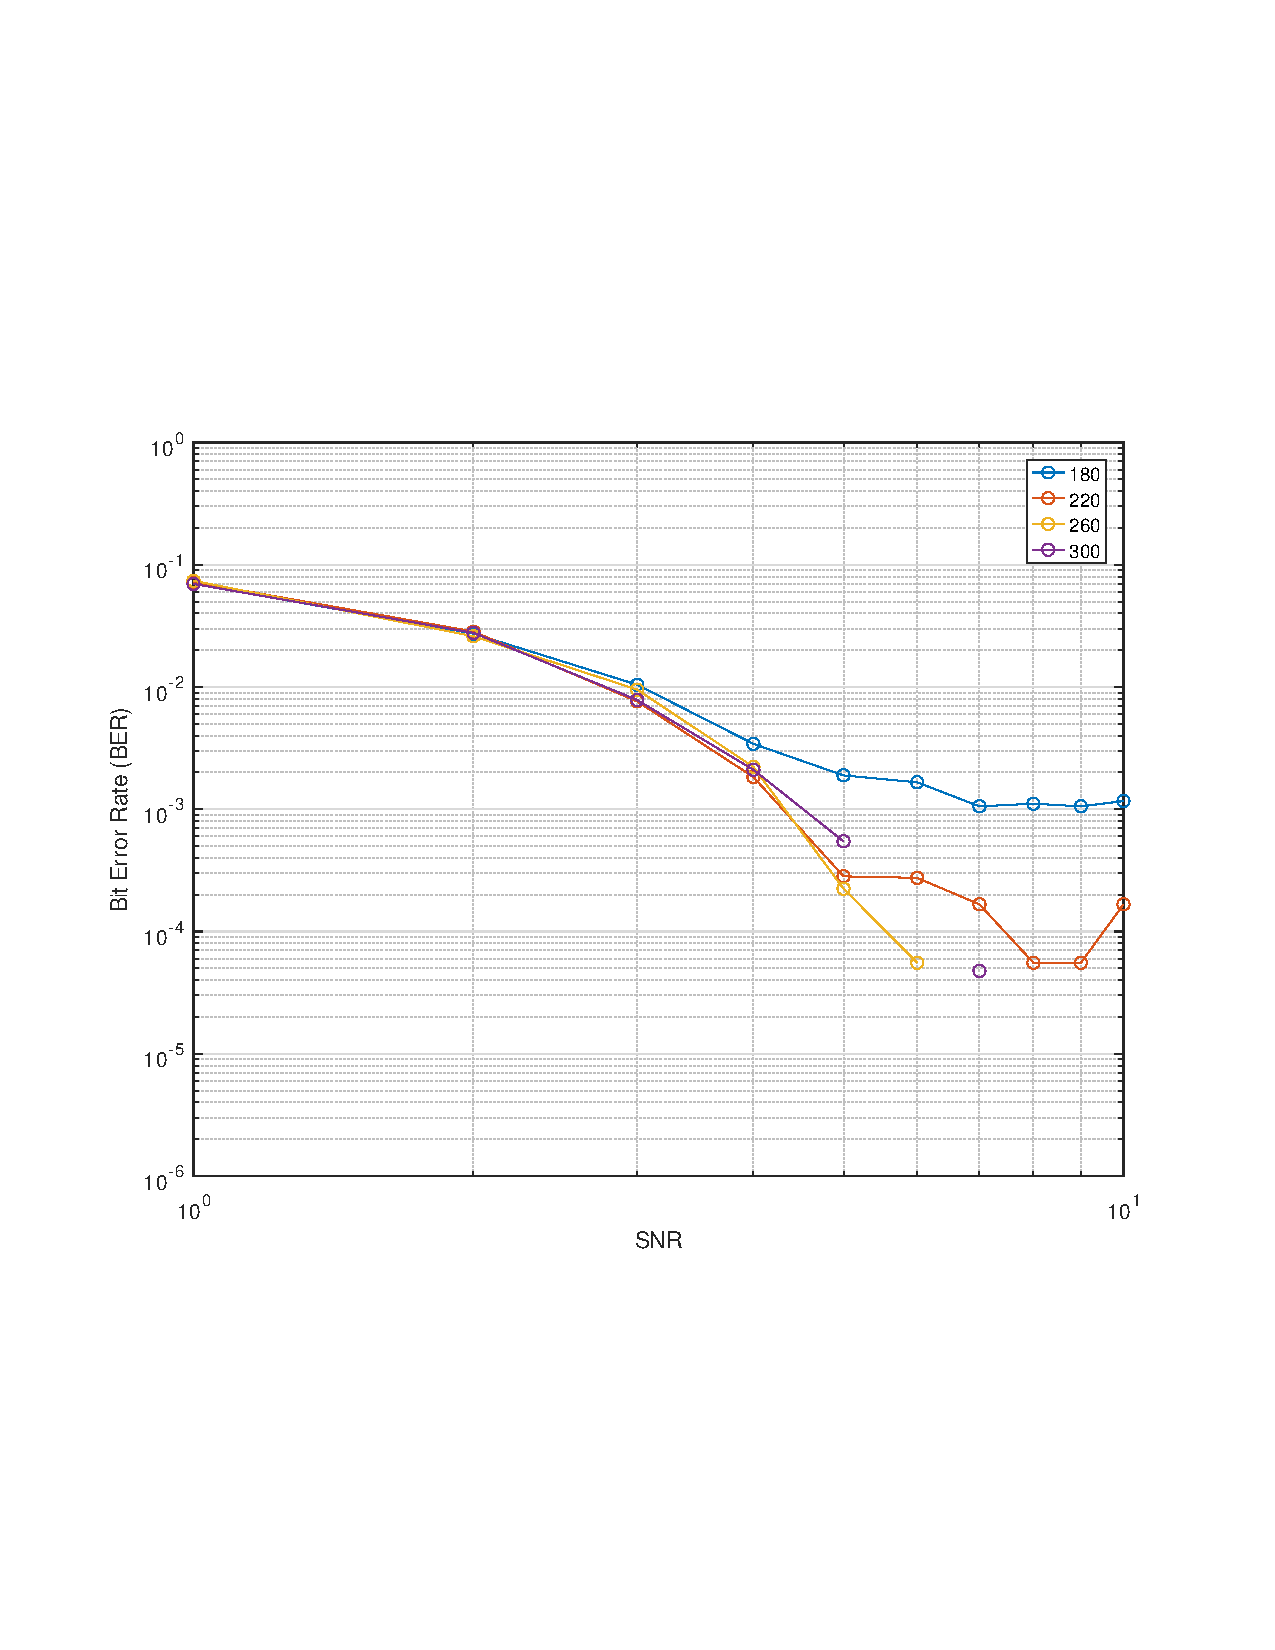
\includegraphics[scale=0.4]{Fountainplot.pdf} 
\caption{Result of AWGN Channel (SNR vs BER)}
\label{AWGN_Channel}
 \end{center}
\vspace{-0.1in}
\end{figure}

\section{Overview}
$Input \to Encoded \to Modulation \to Channel \to Demodulation \to Decoded \to Output
$
\begin{equation*}
\begin{bmatrix}
Code Matrix 
\end{bmatrix}
*  
\begin{bmatrix}
Input
\end{bmatrix} 
= 
\begin{bmatrix}
Encoded Bits 
\end{bmatrix}
\end{equation*}

\begin{equation*}
\begin{bmatrix}
Encoded Bits 
\end{bmatrix} 
\to  
\begin{bmatrix}
Modulated Bits
\end{bmatrix}
\end{equation*}

\begin{equation*}
\begin{bmatrix}
Modulated Bits
\end{bmatrix} 
\to  
\begin{bmatrix}
Channel Error 
\end{bmatrix} 
\end{equation*}

\begin{equation*}
\begin{bmatrix}
Channel Output
\end{bmatrix} 
\to  
\begin{bmatrix}
Demodulated Bits
\end{bmatrix} 
\end{equation*}

\begin{equation*}
\begin{bmatrix}
Code Matrix \vert Demodulated Bits
\end{bmatrix}
\to  
\begin{bmatrix}
Decoded Bits
\end{bmatrix}
\end{equation*}

Compare Decoded Bits with Input Bits, If matches no error if not there is error and then BER is calculated

\end{document}